\chapter{A result on the rate of convergence of the ADMM algorithm}
\label{chap:admm}
\markright{{~{\rm \ref{chap:admm}.A result on the convergence rate of ADMM}}\hfill}{}

\minitoc

\section{Introduction}
\newthought{The ADMM algorithm} \citep{glowinski1975approximation,gabay1976dual,eckstein1992douglas} is
an operator-splitting optimization method which is easy to implement and 
well-adapted for large-scale optimization problems
\citep{boyd2011distributed}. For penalized regression problems with
complicated composite penalties, such as for example analysis sparse
problems \citep{vaiter2013robust},  ADMM can provide a distinctive advantage
over proximal gradient methods such as FISTA \citep{beck09fista} 
when there is no closed-form expression for the 
proximal operator. Indeed, ADMM can
avoid this difficulty by introducing a ``split'' variable, for which the
proximal operator results in updates computable in closed-form.
This is typically the case in \emph{analysis sparsity} regularization,
that impose sparsity on a transformation of the optimization variable. 
However, the theory of the convergence rate of ADMM is
not complete \citep{boyd2011distributed}.

In our ICASSP 2016 paper  \citep{dohmatob2015local}, we studied the convergence of
the ADMM (Alternating Direction Method of Multipliers) algorithm on a broad range of penalized
regression problems including the Lasso, Group-Lasso and Graph-Lasso,(isotropic)
TV-L1, Sparse Variation, and others, that can be written in the form

\begin{equation}
  \underset{(\w,\z) \in \mathbb{R}^p \times
    \mathbb{R}^q}{\text{minimize}}\text{ }\frac{1}{2}\|\X\w-\y\|^2 +
  \lambda\Omega(\z) \text{ subject to }\K\w
    - \z = 0,
  \label{eq:main_pb}
\end{equation}
where $\X \in \mathbb{R}^{n \times  p}$ is the design matrix; $\y \in
\mathbb{R}^n$ is a vector of measurements or classification targets; 
$\K\in\mathbb{R}^{q \times p}$ is linear operator;  $\lambda > 0$ is the
regularization parameter;
and $\Omega: \mathbb{R}^p \rightarrow (-\infty, +\infty]$ is
    the penalty, which is assumed to be a \textit{closed proper
      convex} function.
    In signal processing literature, such a problem is referred to as synthesis problem: the penalty $\Omega$ is imposed not directly on the image, but on a the output of a dictionary, $\z = \K\w$. $\K$ is referred to the analysis operator. The case $\K = \Id$ corresponds to the \textit{synthesis}
    setting.

\subsection{The ADMM algorithms}
Consider the ADMM algorithm
~\citep{glowinski1975approximation,gabay1976dual,eckstein1992douglas,boyd2011distributed}
applied to problem \eqref{eq:main_pb}. Let $\boldsymbol{\mu}\in\mathbb{R}^q$ be
the dual variable %% \footnote{These are Lagrange multipliers.}
and $\nu > 0$ be the penalty parameter on the splitting residual.
%% $\frac{1}{2}\|Kw -\B{z}\|^2$ in the augmented Lagrangian
The augmented Lagrangian is:
\[
\mathcal{L}_{\nu}(\w, \z, \boldsymbol{\mu}) = \frac{1}{2}\|\X\w-\B{y}\|^2 +
  \lambda\Omega(\B{z}) + \boldsymbol{\mu}^T(\B{Kw} -\B{z}) + \frac{1}{2}\nu\|\B{Kw}-\B{z}\|^2.
\]
Further, introducing the scaled dual variable $\u := \nu^{-1}\boldsymbol{\mu}$, which
we will use instead of \(\boldsymbol{\mu}\) from here on, the ADMM iterates for
problem  \eqref{eq:main_pb} are given by the following equations:
\begin{eqnarray}
    \begin{split}
      \B{w}^{(n+1)} &\leftarrow
      \underset{\w}{\argmin}\text{ }\mathcal{L}_{\nu}(\B{w}, \B{z}^{(n)},
      \B{u}^{(n)}) =\\
      &\hspace{.7em}(\nu \B{K}^T\K + \X^T\X)^{-1}(\nu \B{K}^T(\z^{(n)} -
      \B{u}^{(n)}) + \X^T\y)\\\z^{(n+1)} &\leftarrow
      \underset{\z}{\argmin}\text{ }\mathcal{L}_{\nu}(\B{w}^{(n+1)}, \z,
      \B{u}^{(n)}) = \\
      &\hspace{1.3em}\prox_{(\alpha/\nu)\Omega}(\B{Kw}^{(n+1)} + \B{u}^{(n)})\\
      \B{u}^{(n+1)} &\leftarrow \B{u}^{(n)} + \B{Kw}^{(n+1)} -\B{z}^{(n+1)}.
    \end{split}
\label{eq:admm}
\end{eqnarray}

\paragraph*{\textbf{\textit{Assumptions.}}}
We will assume that the matrix sum $\nu
\B{K}^T\K + \X^T\X$ is invertible. This assumption is equivalent to \(\ker
\K^T\K \cap \ker \X^T\X = \{0\}\) (see e.g \cite[Theorem 1]{piziak1999}),
which is  reasonable in the context of regularization. Indeed, the
idea behind this assumption is that, in high-dimensional problems ($n
\ll p$), $\X$ typically has a large kernel, and so one would naturally
choose $\K$ to act on it.

\subsection{Examples}
Problem \eqref{eq:main_pb} covers a broad spectrum of problems
encountered in pattern recognition and image processing. Here are a few:

\paragraph*{Classical examples.}
We have $\Omega = \frac{1}{2}\|.\|^2$ for Ridge regression;
$\Omega = \|.\|_1: z \mapsto \sum_{j \in [p]}|z_j|$
for Lasso and Fused-Lasso ~\citep{Tibshirani05}. For all but the last of
these examples, we have $\K = \Id$. For Group-Lasso, we have $\K=\Id$,
$\Omega = $ the \textit{mixed-norm} $\ell_{2,1}= \|.\|_{2,1}:z
\mapsto \sum_{j \in [\![d]\!]}\|z_{j:j+c-1}\|$, where there are $d \ge
1$ blocks $z_{j:j+c-1}:=(z_j, z_{j+1}, ..., z_{j+c-1})$ each of size $c \ge
1$. %% , giving a total of $d \times c =
%% q$ coordinates).
\label{sec:examples}

\paragraph*{Isotropic TV-L1 and Sparse Variation.}
The different extensions of the TV penalty presented in chapter \ref{chap:structured_priors} can be posed in the form of the problem above.
For example, Sparse Variation~\citep{eickenberg2015total} corresponds to taking
$\K = [\rho\Id,\hspace{.5em}(1-\rho)\nabla]^T \in
\mathbb{R}^{4p \times p}$, where $\nabla$ is the discrete
(refer to chapter \ref{chap:structured_priors}) spatial gradient operator
and $\rho \in [0, 1]$ is a mixing parameter.
For TV-L1 ~\citep{baldassarre2012,gramfort2013}, the penalty is
given by $\Omega(\B{z}) = \sum_{j \in [\![p]\!]}|z_{j,1}| + \sum_{j \in
  [p]}\|z_{j,2:4}\|$ (i.e an $\ell_1$ norm on the first $p$
coordinates of $z$ and an $\ell_{2,1}$ mixed-norm on the last $3p$
coordinates). In particular, the case $\rho = 1$
corresponds to the usual $\ell_1$ norm, while $\rho = 0$ corresponds to
the isotropic TV semi-norm.
% \begin{wrapfigure}{L}{.27\textwidth}
%   \centering
%   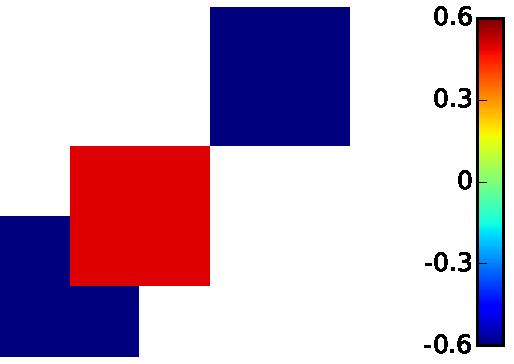
\includegraphics[width=.6\linewidth]{cartoon.pdf}
%   \caption{Structured and sparse weights $w$}
%   \label{fig:roi}
% \end{wrapfigure}

In Sparse Variation ~\citep{eickenberg2015total}, 
the penalty is modified to simply be an $\ell_{2,1}$
mixed-norm on $d = p$ blocks of size $c = 4$ each, i.e
$\Omega(\B{z}) = \sum_{j \in [p]}\|z_{j,1:4}\|$. 
TV-L1 and Sparse Variation combine sparsity (due to the
the $\ell_1$-norm) and structure (due to the isotropic TV term) to
extract local concentrations of spatially correlated features
from the data.%  Fig. \ref{fig:roi} is a good illustration of the
% kinds of patterns one can learn using TV-L1 and Sparse Variation
% models.

% We then showed that this nonlinear operator is
% Fr\'echet-differentiable almost everywhere and that around each fixed
% point, Q-linear convergence is guaranteed, provided the spectral
% radius of the Jacobian of the operator at the fixed point is less than
% 1 (a classical result on stability). Moreover, this spectral radius is
% then a rate of convergence for the ADMM algorithm. Also, we showed that
% the support of the split variable can be identified after finitely
% many iterations. In the anisotropic cases, we show that for
% sufficiently large values of the tuning parameter, we recover the
% optimal rates in terms of Friedrichs angles, that have appeared
% recently in the literature.

\section{Our contributions}
\subsection{Preliminaries}
In the spirit of \citep{ghadimi2013optimal},
let us start with a simple lemma (proof omitted) which
rewrites the ADMM iterates \eqref{eq:admm} as a Picard fixed-point
process in terms of the $(\z, \u)$ pair of variables.%%  This follows from
%% the fixed-point expression of Douglas-Rachford schemes, to which ADMM
%% belongs.

\begin{lemma}
  Define the following objects:
  \begin{eqnarray*}
    \begin{aligned}
      %% Q := \B{X}^T\X \in \mathbb{R}^{p \times p},\hspace{.5em}\Delta :=
      %% \K^T\K \in \mathbb{R}^{p \times p},\hspace{.5em}
      &\G_{\nu} :=
      \K(\K^T\K + \nu^{-1}\B{X}^T\X)^{-1}\K^T,\hspace{.5em}
      \A_{\nu}:=[\G_{\nu}\hspace{.5em}\Id-\G_{\nu}],\\
      &\b_{\nu} := \nu^{-1}\K(\K^T\K +
      \nu^{-1}\B{X}^T\X)^{-1}\B{X}^T\y,\hspace{.2em}\tilde{\A}_{\nu} :=
      \A_{\nu}(.) +  \b_{\nu},\\
      &\Lambda_{\nu} :=
        \left(\prox_{(\alpha/\nu)\varphi}\circ\tilde{\A}_{\nu},
        (\Id-\prox_{(\alpha/\nu)\varphi})\circ\tilde{\A}_{\nu}\right).
    \end{aligned}
    \label{eq:factorize}
  \end{eqnarray*}
 Then the $z$ and $u$ updates in the ADMM iterates
\eqref{eq:admm} can be jointly written as a Picard fixed-point
iteration for the operator $\Lambda_{\nu}$, i.e
\begin{equation}
  (\z^{(n+1)}, \B{u}^{(n+1)}) \leftarrow
  \Lambda_{\nu}(\z^{(n)}, \u^{(n)}).
      \label{eq:fixed_point}
\end{equation}
\label{thm:fixed_point}
\end{lemma}
 In the special case where
$\prox_{(\alpha/\nu)\varphi}$ is a linear transformation --as
in Ridge regression or the nonnegative
Lasso, for example-- the operator $\Lambda_{\nu}$ is linear so that the
fixed-point iteration
\eqref{eq:fixed_point} is a linear dynamical system. Moreover,
in such cases one can derive closed-form formulae for the spectral radius
$r(\Lambda_{\nu})$ of $\Lambda_{\nu}$ as function of $\nu$, and thus recover
the results of \citep{ghadimi2013optimal} and \citep{boley2013}. In the
latter simple situations, a strategy for speeding up the ADMM
algorithm is then to choose the parameter $\nu$ so that the spectral
radius of the linear part of the then affine transformation $\Lambda_\nu$
is minimized. The following Corollary is immediate. Due to lack of
space, we omit the proof, which is obtainable via the \textit{Spectral
  Mapping Theorem}.
\begin{corollary}
  Let $\G_{\nu}$, $\A_{\nu}$, $\tilde{\A}_{\nu}$, and $\Lambda_\nu$ be
  defined as in Lemma \ref{thm:fixed_point}. 
  Then the following hold:
  \begin{itemize}
    \item[\textit{(a)}] $\max(\|\G_\nu\|,
      \|\Id-\G_{\nu}\|) \le 1$,
      $\nu_{\min^*}(\A_\nu) \ge 1/\sqrt{2}$, and $\|\A_{\nu}\| \le 1$
      with equality in the last inequality iff at least one of $\G_\nu$
      and $\Id-\G_\nu$ is singular.
\item[\textit{(b)}] $\Lambda_\nu$ is $\|\A_\nu\|$-Lipschitz. That is,
  $\forall (\x_1, \x_2) \in \mathbb{R}^{q+q} \times \mathbb{R}^{q+q}$,
\begin{eqnarray}
  \|\Lambda_{\nu}(\x_1) - \Lambda_\nu(\x_2)\| \le
  \|\A_\nu\|\|\x_1 - \x_2\|.
  \label{eq:tight}
\end{eqnarray}
 In particular, if $\|\A_\nu\| < 1$,
  then $\Lambda_\nu$ is a contraction and the ADMM
  iterates \eqref{eq:admm} converge globally Q-linearly to a
  solution of \eqref{eq:main_pb}. Moreover, this solution is unique.
  \end{itemize}
\label{thm:fixed_point_corr}
\end{corollary}

According to Corollary \ref{thm:fixed_point_corr}, $\Lambda_\nu$ is an
$\|\A_\nu\|$-contraction in case $\|\A_\nu\| < 1$, and so we have
global Q-linear convergence of the ADMM iterates \eqref{eq:admm} at the
rate $\|\A_\nu\|$. This particular case is analogous to the results
obtained in \citep{nishihara2015general} when the loss function or the
penalty is strongly convex.
But what if $\|\G_\nu\| = \|\Id-\G_\nu\| =
\|\A_\nu\| = 1$ ? Can we still have Q-linear convergence, --at
least locally ? These questions are answered in the sequel.

\subsection{Behavior of ADMM around fixed-points}
\begin{marginfigure}[4cm]
  \label{fig:rates}  
  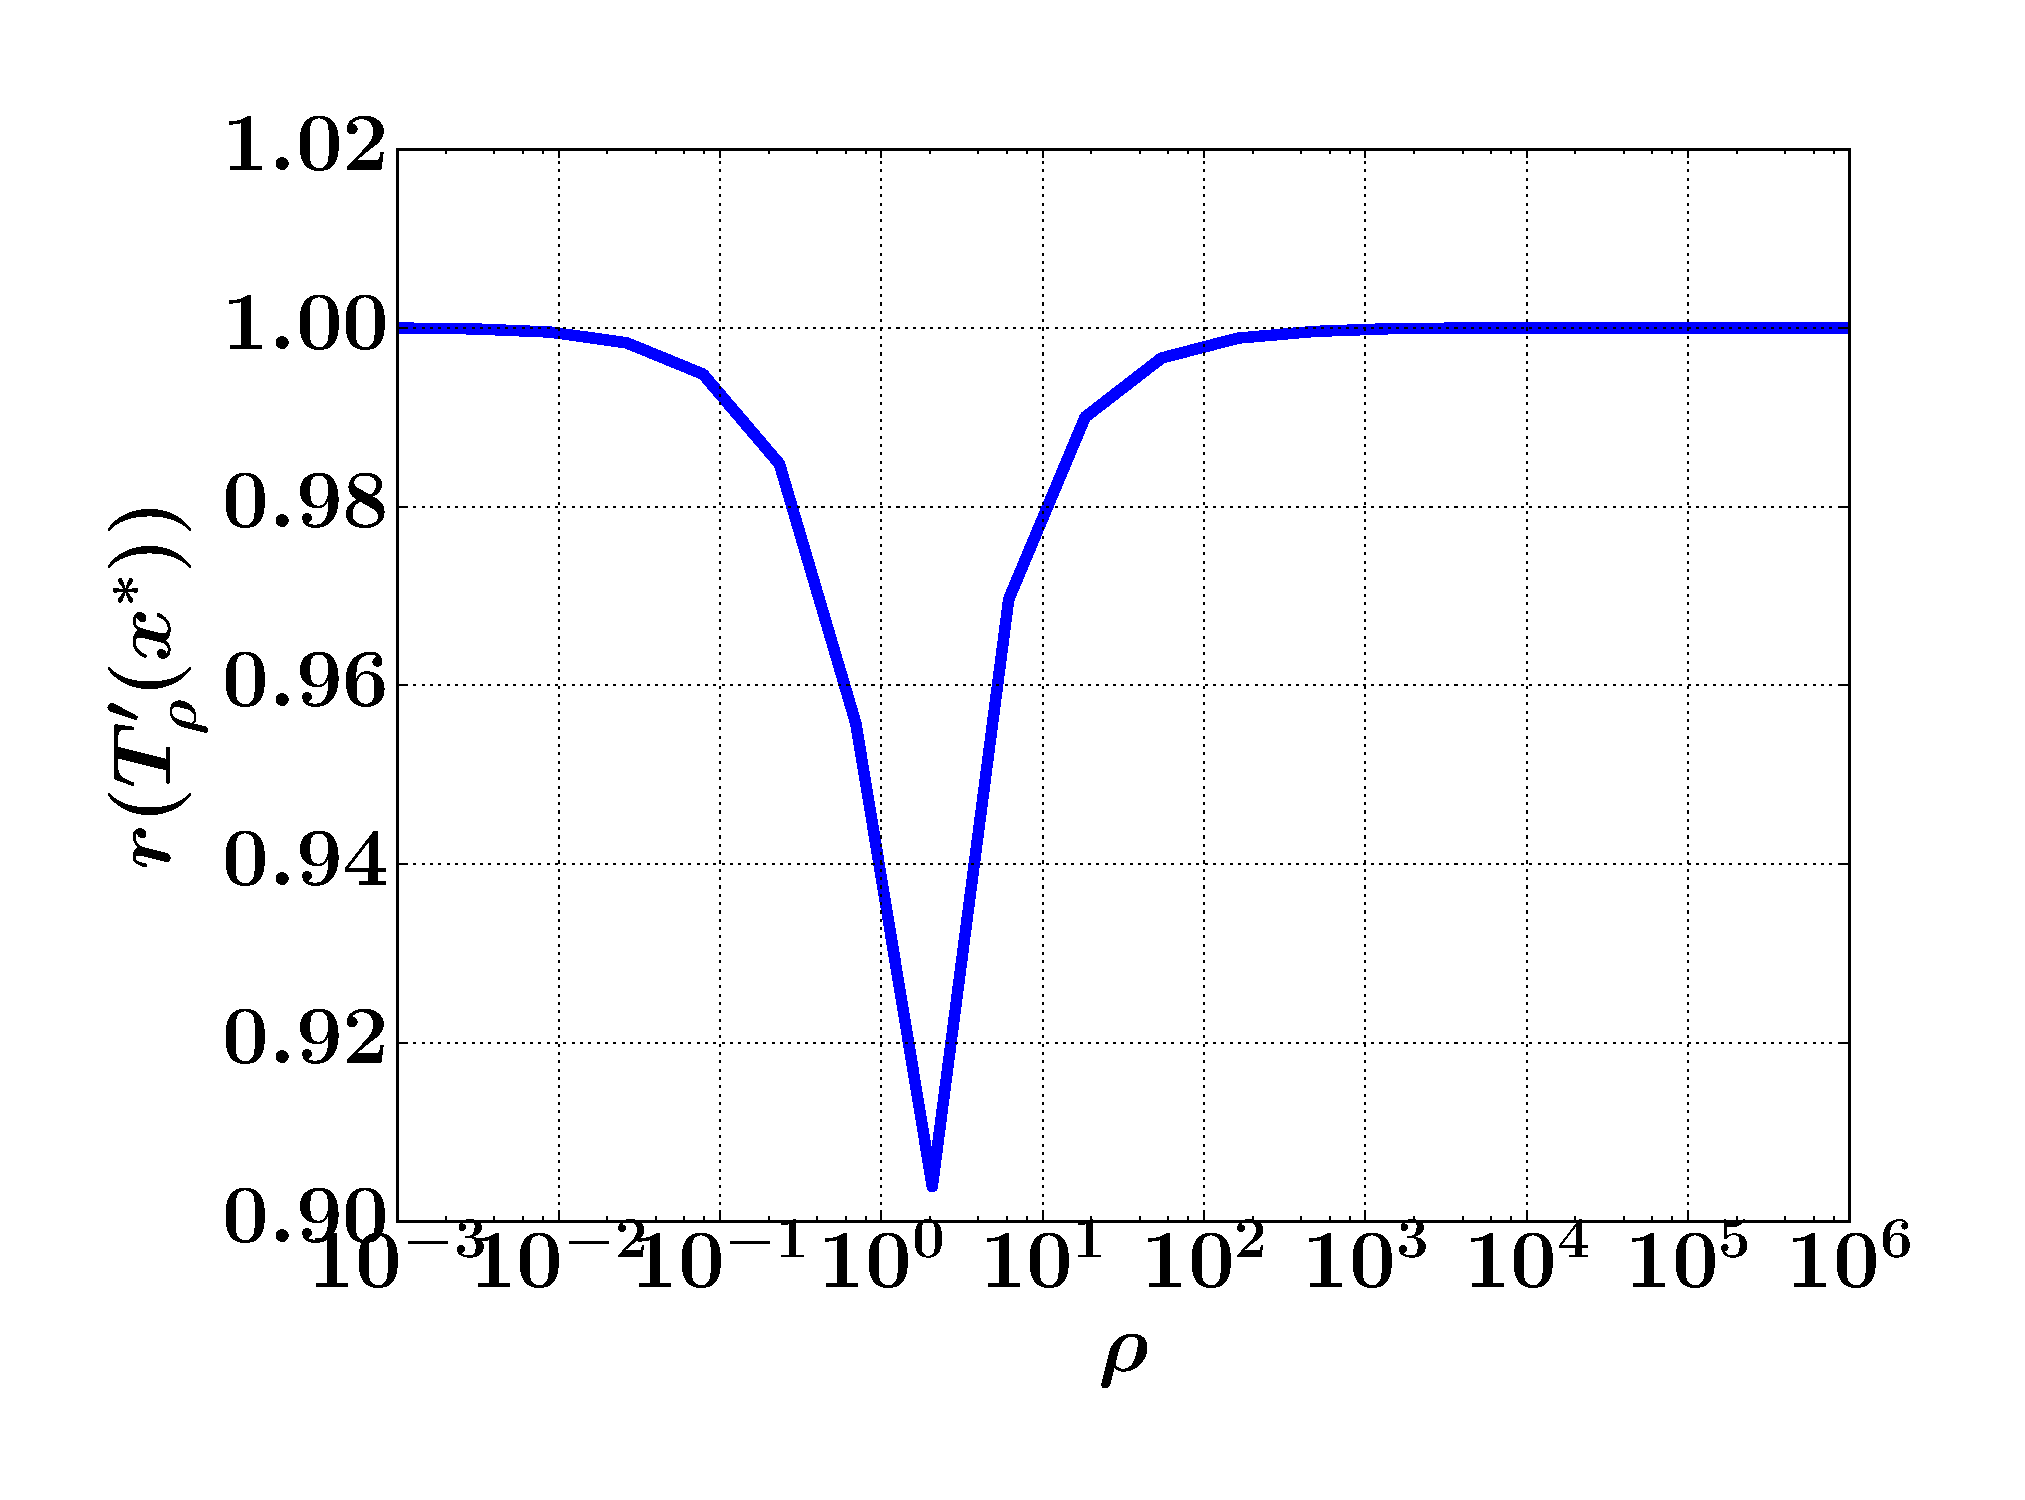
\includegraphics[width=1.2\linewidth]{figures/lasso_rates.pdf}%
\caption{Rate of convergence $r(\Lambda'_\nu(\x^*))$ as a function of $\nu$
  for a Lasso problem with column-rank deficient design
  matrix $\X$. Taking $\nu$ too small leads
  to badly conditioned problem (as  $\Id + (1/\nu)\B{X}^T\X$ is then almost
  singular), and thus a slow rate of convergence (near 1). On the
  other hand, the figure suggests that taking $\nu$ ``too large''
  is also detrimental. Most remarkable, one notices that the basin of
  ``good'' $\nu$ values is rather tight, and so care must be taken in
  choosing the $\nu$ parameter.
}
\end{marginfigure} %-----------------------------------------------------------

Henceforth, we consider problem \eqref{eq:main_pb} in situations
where the penalty $\varphi$ is an $\ell_{2,1}$
mixed-norm. Note that the $\ell_1$-norm is a special case of the
$\ell_{2,1}$ mixed-norm with $c=1$ feature per block, and corresponds
to the anisotropic case. The results presented in Theorem
\eqref{thm:frechet} carry over effortlessly to the case where the
$\varphi$ is the
  concatenation of $\ell_{2,1}$ norms, for example as in the the TV-L1
  semi-norm. %%  $\varphi(K\cdot)$, where $\B{Kw} \equiv ((1-\rho)
  %%   \nabla(w),\hspace{.5em}\rho w)$ and $\varphi = (\ell_{2,1},
  %% \ell_1)$.
  %% Also, part \textit{(b)} of \ref{thm:frechet} can be
  %% extended to even more general instances of problem
  %% \eqref{eq:main_pb} for which the proximal operator of the penalty
  %% function $\varphi$ is is differentiable everywhere except some
  %% ``degenerate'' points.
The following theorem --inspired by a careful synthesis of
the arguments in \citep{holmes1973} and \citep{bayram2010subband}--
is our main result.

Our main results are summarized in Theorem 1 of the aforementioned paper, which we now state.
\begin{theorem} Consider the ADMM algorithm \eqref{eq:admm} on problem
  \eqref{eq:main_pb}, where $\Omega$ is an $\ell_{2,1}$ mixed-norm on
  $d \ge 1$ blocks each of size $c \ge 1$, for a total of $q = d
  \times c$ features. Let the operators $\B{A}$, $\tilde{\B{A}}$, and $\Lambda$ be
  defined as defined above, with the $\nu$ subscript
  dropped for ease of notation. Let For $\B{x} = (\B{z}, \B{u}) \in\mathbb{R}^{q+q}$, let $\Lambda_1(\B{x}) \in \mathbb R^q$ denote the first $q$ coordinates of $\Lambda(\B{x})$, i.e its $z$-part. Define
  \begin{itemize}
    \item $\supp(\B{z}) := \{j\in[\![d]\!]\text{ }|\text{ }z_{j:j+c-1} \ne
      0\}$;
      \item $\mathcal{A}_1(\B{z}) := \{\B{z}' \in \mathbb{R}^{q} |
    \supp(\B{z}') = \supp(\B{z})\}$, and $\mathcal A(\B{x}) := \mathcal A_1(\B{z}) \oplus \mathbb R^q$;
   \item $\tilde{\B{x}} := (\tilde{\B{x}}_j)_{j \in [\![d]\!]} := \tilde{\A}\B{x}$, $\kappa :=
    \alpha / \nu$, $\epsilon(\B{x}) :=
      \underset{j \in [\![d]\!]}{\min}\text{}|\|\tilde{\B{x}}_j\|-\kappa| \ge 0$.
    \end{itemize}
Then the following hold:
\begin{itemize}
\item[\textit{(a)}] \textbf{Attractivity of supports.} For all $\B{x} \in
  \mathbb{R}^{q+q}$, we have
  \[\Lambda(\bar{\mathbb{B}}_{2q}(\B{x},\epsilon(\B{x})/\|\A\|)) \subseteq
  \bar{\mathbb{B}}_{2q}(\Lambda(\B{x}),\epsilon(\B{x})) \cap
  \mathcal{A}(\Lambda(\B{x})).\] In
  particular, if $\B{x}^*$ is a fixed-point of the operator $\Gamma$, then
  \[
  \Lambda(\bar{\mathbb{B}}_{2q}(\B{x}^*,\epsilon(\B{x}^*)/\|\A\|))
  \subseteq
  \bar{\mathbb{B}}_{2q}(\B{x}^*,\epsilon(\B{x}^*)) \cap \mathcal{A}(\B{x}^*).
  \]
\item[\textit{(b)}] \textbf{Fr\'echet-differentiability.} If $\B{x} \in
  \mathbb{R}^{q+q}$ with
  $\epsilon(\B{x}) > 0$, then $\Lambda$ is Fr\'echet-differentiable at $\B{x}$ with
  derivative
\begin{eqnarray}
  \Lambda'(\B{x}) = \B{F}_{\B{x}}\A \in \mathbb{R}^{2q \times 2q},
\label{eq:linear}
\end{eqnarray}
where $\B{F}_{\B{x}} := [\B{D}_{\B{x}} \hspace{.6em} \Id - \B{D}_{\B{x}}]^T$ and  $\B{D}_{\B{x}} \in
\mathbb{R}^{q \times q}$ is a block-diagonal matrix
with block $\B{D}_{\B{x},j} \in \mathbb{R}^{c \times c}$
given by
\begin{eqnarray}
\B{D}_{\B{x},j} = \begin{cases}\Id -
  \frac{\kappa}{\|\tilde{\B{x}}_j\|}P_{\langle
        \tilde{\B{x}}_j \rangle^\perp}, &\mbox{ if } j \in
  \supp(\Lambda_1(\B{x})),\\ 0, &\mbox{ otherwise.}\end{cases}
\label{eq:d}
\end{eqnarray}
In particular,  when $c=1$,  each $\B{D}_{\B{x}^,j}$ reduces to a
bit $\in \{0,1\}$ which indicates whether the $j$th feature is
active, and $\B{D}_{\B{x}}$ reduces to a diagonal projector matrix with only
0s and 1s.

\item[\textit{(c)}] Let $\B{x}^* = (\B{z}^*, \B{u}^*)\in \mathbb{R}^{q+q}$ be any fixed-point of $\Gamma$.
\begin{itemize}
\item[\textit{(1)}] \textbf{Finite-time identification of
    active set.} If the closed ball $\bar{\mathbb{B}}_{2q}(\B{x}^*, \epsilon(\B{x}^*)/\|\A\|)$
    contains any point of the sequence of iterates $x^{(n)}$, then the
    active set $\mathcal{A}(\B{x}^*)$ is
    identified after finitely many iterations, i.e
    \begin{eqnarray}
      \label{eq:id}
      \exists N_{\B{x}^*} \ge 0 \text{ s.t }\B{x}^{(n)} \in \mathcal{A}(\B{x}^*)
      \forall n \ge N_{\B{x}^*}.
    \end{eqnarray}
      In particular, \eqref{eq:id} holds if $\B{x}^{(n)}$ converges to $\B{x}^*$.

\item[\textit{(2)}] \textbf{Local Q-linear convergence.}
If $\epsilon(\B{x}^*) > 0$ and $r(\Lambda'(\B{x}^*)) < 1$, then the iterates
$x^{(n)}$ converge locally Q-linearly to $\B{x}^*$
at the rate $r(\Lambda'(\B{x}^*))$.

\label{thm:frechet}
\item[\textit{(3)}] \textbf{Optimal rates in the anisotropic case.}
If $c=1$ (as in anisotropic TV deconvolution) and $\nu$ is large, then the optimal rate of convergence
rate is the cosine of the Friedrichs angle between
$\mathrm{Im}\;\K$ and $\mathrm{Im}\;\B{D}_{\B{x}^*} \simeq \mathcal A_1(\B{z}^*)$. If in addition
$K = \Id$ (as in synthesis inverse problems like the Lasso, sparse  Spike-deconvolution, etc.), then
the whole algorithm converges in a finite number of iterations.
\end{itemize}
\end{itemize}
\end{theorem}

\begin{proof}
  See our ICASSP paper ~\citep{dohmatob2015local}.
\end{proof}

\section{Relation to prior work}
\label{sec:lit}
Recently, there have been a number of results on the local
linear convergence of ADMM on particular classes of problems. Below,
we outline the corresponding major works.

\subsection{{Ridge, QP, and nonnegative Lasso}} On problems like
Ridge regression, quadratic programming (QP), and
nonnegative Lasso, \citep{ghadimi2013optimal} demonstrated local linear
convergence of ADMM under certain rank conditions which
are equivalent to requiring that the p.s.d matrix $\G_\nu$ (defined in
\eqref{eq:fixed_point}) be invertible. The same paper
prescribed explicit formulae for optimally selecting the tuning
parameter $\nu$ for ADMM on these problems. %% It shows the
We note that these results can be recovered from our Lemma
\ref{thm:fixed_point} and Corollary \ref{thm:fixed_point_corr} as they
correspond to the case where
$\prox_{(\alpha/\nu)\varphi}$ is a linear operator. Using
similar spectral arguments, \citep{boley2013} demonstrated similar
local convergence results for quadratic and linear QP problems.

\subsection{{Fr\'echet-differentiable nonlinear systems}} In the SISTA
algorithm \citep{bayram2010subband},
the authors linked the rate of convergence of their multi-band
ISTA (refer to \citep{daubechies2004} and the references therein,
for the original ISTA algorithm)
 scheme to the spectral radius of a certain Jacobian matrix related to
 the problem data and dependent on the fixed-point \cite[Propositions
   6 and  7]{bayram2010subband}, provided this spectral radius is less
 than 1.
Most importantly, the authors show \cite[Proposition
   8]{bayram2010subband} how their algorithm can be made as fast as
 possible by choosing the shrinkage parameter per sub-band to be ``as
 large as possible''. Finally, analogous to our Theorem
\ref{thm:frechet}\textit{(a)}, Lemma 2 of \citep{bayram2010subband}
shows that the SISTA iteration projects points sufficiently close to
fixed-points onto the support of these fixed-points. 

\subsection{{Partly-smooth functions and Friedrichs angles}} In the
recent work \citep{liang2014activity} which focuses on
Douglas-Rachford/ADMM, and \citep{liang2015activity} which
uses the same ideas as in \citep{liang2014activity} but with a
forward-backward scheme \citep{combettes2005signal},
the authors consider a subclass PSS (refer to definition 2.2 of
  \citep{liang2015activity}) of the class of so-called partly-smooth
  (PS) penalties
% (these include the $\ell_1$,
% $\ell_{2,1}$, and $\ell_\infty$ norms)
and general $\mathcal C^2$ loss functions with Lipschitz
gradient. Under nonlinear complementarity requirements analogous to
the non-degeneracy assumption ``$\epsilon(\x^*) > 0$'' of Theorem
\ref{thm:frechet}\textit{(b)}, and rank constraints analogous to the
requirement that the Jacobian matrix $\Lambda'(\x^*)$
have spectral radius less than 1 (in Theorem
\ref{thm:frechet}\textit{(c2)}), the authors of
\citep{liang2014activity,liang2015activity} prove finite-time activity
identification and local Q-linear convergence at a rate given in terms of
\textit{Friedrichs angles}, via direct application of \cite[Theorem
3.10]{bauschke2014optimal}.
The authors show that their
arguments are valid for a broad variety of problems, for example the
\textit{anisotropic} TV penalty. %% More on this comparison in
%% \ref{sec:longterm}.
Still in the
framework of partly-smooth penalties, \citep{demanet2013eveventual}
showed local Q-linear convergence of the Douglas-Rachford algorithm on
the Basis Pursuit problem.

\paragraph*{Detailed comparison with
  \citep{liang2014activity,liang2015activity}.} The
works which are most comparable to ours are \citep{liang2014activity}
and \citep{liang2015activity}, already presented above. Let us point
out some similarities and differences between these papers and
ours. First, though our constructions are entirely different from the
techniques developed in
\citep{liang2014activity,liang2015activity}, one notes that both
approaches are ultimately rooted in
the same idea, namely
the work of B. Holmes \citep{holmes1973} on the smoothness of the euclidean
projection onto convex sets, and other related functionals (Minkowski
gauges, etc.). Indeed, Theorem \ref{thm:frechet} builds
directly upon \citep{holmes1973}, whilst, \citep{liang2015activity} and
\citep{liang2014activity} are linked to \citep{holmes1973} via
\citep{wright93}, which builds on \citep{phelps82}, and the latter builds
on \citep{holmes1973}.

Second, part \textit{(c1)} of Theorem \ref{thm:frechet} (finite-time
identification of active set) of the theorem can be recovered as a
consequence of the results established in
\citep{liang2014activity,liang2015activity}. However, the rest of our
results, notably part \textit{(c2)} (Q-linear convergence) cannot be
recovered from the aforementioned works, at least on models like
isotropic TV-L1, Sparse Variation, etc., since these models are not
PSS. Indeed, the convergence rates in
\citep{liang2014activity,liang2015activity} do not extend from
anisotropic to isotropic TV, for example. Success in the former case
is due to the fact that the anisotropic TV semi-norm is polyhedral
and therefore is of class PSS at each point. By contrast, our framework
can handle isotropic TV and similar ``entangled'' penalty types like
isotropic TV-L1, Sparse Variation, etc., but suffers complementary
limitations; for example, 
we were unable to generalize it
beyond the squared-loss setting and we can only handle penalties which
are a composition of a $\ell_{2,1}$ mixed-norm (or a concatenation of
such)  and a linear operator. The recent work ~\citep{vaiter2016degrees} on counting the degrees of freedom of general partly-smooth penalties is worth mentioning and may contain some key ideas to help bridge the ``isotropicity gap `` in the methods developed in \citep{liang2014activity,liang2015activity}, concerning rates of convergence.

Lastly, the convergence rates in
\citep{liang2014activity,liang2015activity}
are tight and given in terms of Friedrichs angles
\citep{bauschke2014optimal}, whilst our rates
are given in terms of spectral radii, and will be
suboptimal in certain cases. An exception are the anisotropic cases,
where we proved in part \textit{(c3)} of Theorem \ref{thm:frechet} that
we recover the optimal rates obtained in
\citep{liang2014activity,liang2015activity} in terms of Friedrichs
angles. Moreover, for the Lasso, we showed that the whole algorithm
converges after only finitely many iterations.

\section{Numerical experiments and results}
\label{sec:exp}
Here, we present results for a variety of experiments. Each experiment
is an instance of problem \eqref{eq:main_pb} with an
appropriate choice of the linear operators $\X$, $\K$,  and the penalty
function $\varphi$ which can be the $\ell_1$-norm the
$\ell_{2,1}$ mixed-norm, or a mixture of the two (as in TV-L1).

\paragraph{Setting.}
We use a grid of $20$ values of $\nu$, evenly spaced in
log-space from $10^{-3}$ to $10^6$. For each problem model (see below),
the iteration process \eqref{eq:fixed_point} is started with $\x^{(0)} = 0
\in \mathbb{R}^{q \times q}$, and iterated $N=1500$ times. The final
point $\x^{(N)}$ is approximately a fixed-point $\x^{(*)}$ of the operator
$\Lambda_\nu$. Now, the iteration process is run again (starting with the same
initial $\x^{(0)}$) and the distance $\|\x^{(k)} - \x^{(N)}\|$ is
recorded on each iteration $k$, producing a curve. This procedure is
run for each value of $\nu$ from the aforementioned grid.
Except otherwise stated, the $n$ rows of design matrix $X$ where drawn
from a $p$-dimensional standard Gaussian. The measurements variable
$\y$ is then computed as $\y = \X\w_0 + \textrm{noise}$, where
$\w_0$ is the true signal.

\paragraph{Simple models.}
As discussed in section \ref{sec:lit}, the local Q-linear convergence
of ADMM on a variety of particular problems has been studied in the
literature (for example
\citep{ghadimi2013optimal,nishihara2015general,liang2014activity,liang2015activity}).
We validated empirically our linear convergence
results (Theorem \ref{thm:frechet}) by reproducing experiments from
\citep{liang2014activity,liang2015activity}. For each of these experiments
the regularization parameter $\alpha$ was set to $1$. Viz,

\begin{itemize}
\item[\textit{(a)}] Lasso: Here the problem is an instance of
  \eqref{eq:main_pb} with $\K = \Id$ and $\varphi = \|\cdot\|_1$; $n =
  32$, $q=p=128$, and $w_0$ is 8-sparse.
\item[\textit{(b)}] Group-Lasso: Here $\K = \Id$ and $\varphi =
  \|\cdot\|_{2,1}$, $n = 48$, $p=128$, number of blocks $d=32$, block
  size = $c=4$, $q = d \times c = 128$, $w_0$ is has $2$ non-zero blocks.
\item[\textit{(c)}] Sparse spikes deconvolution: Here, $\K=\Id$, $\X$ is
  a projector  onto low Fourier frequencies (Dirichlet kernel) and the
  penalty $\varphi$ is the $\ell_1$-norm; $n=p=200$ (with $\rank \X =
  40$). The true signal $w_0$ is a 20-sparse vector (of length $p$),
  containing randomly distributed spikes with Gaussian values at a
  minimum pairwise distance of 5.
%% \item[\textit{(d)}] deblurring: ...
\end{itemize}

\begin{pagefigure}
  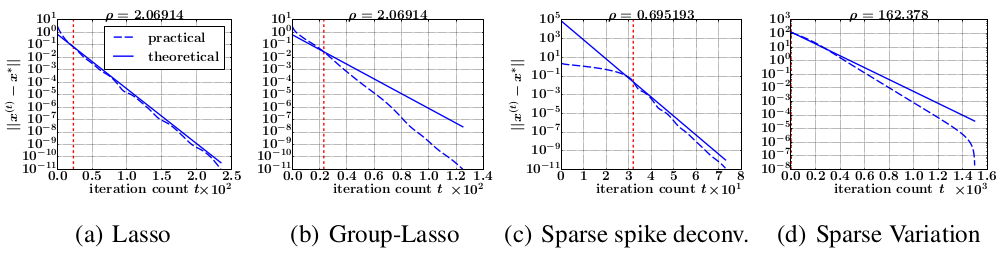
\includegraphics[width=1\linewidth]{figures/admm.png}
  \caption{{Experimental results from ICASSP paper}~\citep{dohmatob2015local}\textbf{.} showing local Q-linear convergence for ADMM
    on problem \eqref{eq:main_pb}. %% Results for
  %% all the other values of $\nu$ are provided in the supplementary matrials.
    The ``theoretical'' line is the exponential
    curve $t \mapsto \|\x^{(0)} - \x^*\|r(\Lambda'(\x^*))^t$. The red broken
    vertical line marks the instant the support of the fixed-point $\x^*$
  % = (\z^*,\u^*)$
    is identified.
  }
\end{pagefigure}

\section{Concluding remarks}
We have derived a fixed-point iteration which is equivalent to the
ADMM iterates for a broad class of penalized regression problems
\eqref{eq:main_pb}. Exploiting the formulation so obtained, we  have
established detailed qualitative properties of the algorithm around
solution points (Theorem \ref{thm:frechet}). Most importantly, under
mild conditions, local
Q-linear convergence is guaranteed and we have provided an explicit
formula for this rate of convergence. %% As can be seen in Fig. \ref{fig:rates},
Finally, Theorem \ref{thm:frechet} --implicitly--
opens the possibility of speeding up the ADMM algorithm on problem
\eqref{eq:main_pb} by selecting the tuning parameter $\nu$ so as to
minimize the spectral radius (an inverted mexican-hat-shaped curve, as
$\nu$ varies from $0$ to $+\infty$) of the Jacobian matrix
$T'_\nu(\x^*)$.

\bibliographystyle{plainnat}
\bibliography{bib_all}

